\chapter{Simulink Code Generation}
\label{app:simulink-codegen}
\index{Simulink!code generation|(}
\index{code generation!Simulink|(}

Model-based development promises that we can design, simulate, and verify control systems using graphical models, then automatically generate production code for embedded targets. This appendix explains how Simulink's code generation works and what the generated code looks like, helping you understand and integrate auto-generated code into your embedded projects.

\section{Introduction: From Model to Embedded Code}

Throughout this course, you have developed Simulink models for quadrotor control---attitude controllers, position estimators, and sensor fusion algorithms. These models run in MATLAB's simulation environment, where numerical integration happens on your laptop with essentially unlimited computational resources. But the ultimate goal is to run these controllers on the Crazyflie's STM32 microcontroller, executing in real-time with strict timing constraints.

\subsection{Why Code Generation?}

You could manually translate your Simulink model into C code, but this approach has significant drawbacks:

\begin{itemize}
    \item \textbf{Error-prone}: Manual translation introduces bugs, especially for complex algorithms
    \item \textbf{Time-consuming}: Re-implementing after every model change is tedious
    \item \textbf{Traceability lost}: No automatic link between model and code
    \item \textbf{Verification burden}: Must re-verify code matches model behavior
\end{itemize}

Automatic code generation addresses these issues by producing C code directly from your Simulink model. The generated code is:

\begin{itemize}
    \item \textbf{Correct by construction}: Mathematically equivalent to the model
    \item \textbf{Traceable}: Every line of code maps to a model element
    \item \textbf{Consistent}: Regenerated automatically when the model changes
    \item \textbf{Verifiable}: Same code used in simulation and on target
\end{itemize}

\begin{keyidea}
Code generation transforms your verified simulation model into deployable embedded software, preserving the design intent and enabling systematic verification through the development process.
\end{keyidea}

\subsection{The V-Model and Code Generation}

Code generation fits into the V-model development process that structures safety-critical system development:

\begin{center}
\begin{tikzpicture}[scale=0.9, every node/.style={font=\small}]
    % Left side - design
    \node[draw, rectangle, minimum width=3cm, minimum height=0.8cm] (req) at (0,4) {Requirements};
    \node[draw, rectangle, minimum width=3cm, minimum height=0.8cm] (arch) at (-1.5,3) {Architecture};
    \node[draw, rectangle, minimum width=3cm, minimum height=0.8cm] (design) at (-3,2) {Detailed Design};
    \node[draw, rectangle, minimum width=3cm, minimum height=0.8cm, fill=blue!10] (model) at (-4.5,1) {Simulink Model};
    \node[draw, rectangle, minimum width=3cm, minimum height=0.8cm, fill=green!10] (code) at (-4.5,0) {Generated Code};

    % Right side - verification
    \node[draw, rectangle, minimum width=3cm, minimum height=0.8cm] (systest) at (1.5,3) {System Test};
    \node[draw, rectangle, minimum width=3cm, minimum height=0.8cm] (inttest) at (3,2) {Integration Test};
    \node[draw, rectangle, minimum width=3cm, minimum height=0.8cm] (unittest) at (4.5,1) {Unit Test};

    % Arrows
    \draw[-{Stealth}] (req) -- (arch);
    \draw[-{Stealth}] (arch) -- (design);
    \draw[-{Stealth}] (design) -- (model);
    \draw[-{Stealth}, thick, blue!60] (model) -- node[right] {Code Gen} (code);

    \draw[dashed, -{Stealth}] (req) -- (systest);
    \draw[dashed, -{Stealth}] (arch) -- (inttest);
    \draw[dashed, -{Stealth}] (design) -- (unittest);

    % Bottom
    \draw[-{Stealth}] (code) -- ++(2,0) -- ++(0,0.5);
    \draw[-{Stealth}] (4.5,0.5) -- (unittest);
\end{tikzpicture}
\end{center}

The Simulink model serves as both the detailed design specification and the source for implementation. Code generation (shown in blue) automatically produces the implementation, while the verification activities on the right side confirm that requirements are met.

\subsection{Simulink Coder vs Embedded Coder}

MathWorks offers two code generation products:

\begin{itemize}
    \item \textbf{Simulink Coder}\index{Simulink Coder}: Generates portable ANSI C/C++ code suitable for rapid prototyping and simulation acceleration. The generated code may use dynamic memory allocation and floating-point arithmetic.

    \item \textbf{Embedded Coder}\index{Embedded Coder}: Extends Simulink Coder with optimizations for production embedded systems. Generates more efficient code with options for fixed-point arithmetic\index{fixed-point arithmetic}, static memory allocation, and compliance with coding standards like MISRA C\index{MISRA C}.
\end{itemize}

For the Crazyflie project, Embedded Coder is preferred because it produces code optimized for resource-constrained microcontrollers and supports the STM32's hardware floating-point unit.

\section{The Code Generation Workflow}

Understanding the code generation workflow helps you configure the process correctly and troubleshoot issues when they arise.

\subsection{From Model to Binary}

The complete workflow from Simulink model to running firmware involves several stages:

\begin{center}
\begin{tikzpicture}[node distance=1.8cm, every node/.style={font=\small}]
    \node[draw, rectangle, rounded corners, fill=blue!10, minimum width=2.5cm, minimum height=1cm, align=center] (model) {Simulink\\Model};
    \node[draw, rectangle, rounded corners, fill=yellow!10, minimum width=2.5cm, minimum height=1cm, right of=model, xshift=1.5cm, align=center] (tlc) {Target\\Language\\Compiler};
    \node[draw, rectangle, rounded corners, fill=green!10, minimum width=2.5cm, minimum height=1cm, right of=tlc, xshift=1.5cm, align=center] (ccode) {Generated\\C Code};
    \node[draw, rectangle, rounded corners, fill=orange!10, minimum width=2.5cm, minimum height=1cm, right of=ccode, xshift=1.5cm, align=center] (compiler) {Cross\\Compiler};
    \node[draw, rectangle, rounded corners, fill=red!10, minimum width=2.5cm, minimum height=1cm, right of=compiler, xshift=1.5cm,align=center] (binary) {Binary\\(.elf)};

    \draw[-{Stealth}, thick] (model) -- (tlc);
    \draw[-{Stealth}, thick] (tlc) -- (ccode);
    \draw[-{Stealth}, thick] (ccode) -- (compiler);
    \draw[-{Stealth}, thick] (compiler) -- (binary);

    \node[below of=model, yshift=0.5cm, font=\scriptsize] {.slx file};
    \node[below of=ccode, yshift=0.5cm, font=\scriptsize] {.c, .h files};
    \node[below of=binary, yshift=0.5cm, font=\scriptsize] {ARM executable};
\end{tikzpicture}
\end{center}

\begin{enumerate}
    \item \textbf{Model Analysis}: Simulink analyzes block connections, sample times, and data types
    \item \textbf{Code Generation}: The Target Language Compiler (TLC)\index{Target Language Compiler (TLC)} produces C source files
    \item \textbf{Compilation}: A cross-compiler (arm-none-eabi-gcc) compiles for the target
    \item \textbf{Linking}: Object files link with runtime libraries and startup code
    \item \textbf{Deployment}: The binary is flashed to the microcontroller
\end{enumerate}

\subsection{Solver Selection for Embedded Targets}

One of the most important configuration choices is the solver. Simulink offers two categories:

\begin{itemize}
    \item \textbf{Variable-step solvers} (ode45, ode23, etc.): Adapt step size based on error estimates. Excellent for simulation accuracy but unsuitable for real-time execution because execution time varies unpredictably.

    \item \textbf{Fixed-step solvers}\index{fixed-step solver} (ode4, ode1, discrete): Take constant-size steps. Required for real-time execution because they guarantee predictable timing.
\end{itemize}

\begin{warningbox}
For embedded targets, you \textbf{must} use a fixed-step solver. Variable-step solvers cannot guarantee real-time deadlines and will cause code generation to fail or produce unsuitable code.
\end{warningbox}

Common fixed-step solver choices:

\begin{center}
\begin{tabular}{lll}
\toprule
\textbf{Solver} & \textbf{Method} & \textbf{Use Case} \\
\midrule
\texttt{ode1} & Euler & Simple, fast, less accurate \\
\texttt{ode2} & Heun & Better accuracy than Euler \\
\texttt{ode4} & Runge-Kutta 4 & Good accuracy, more computation \\
\texttt{discrete} & No integration & Purely discrete-time models \\
\bottomrule
\end{tabular}
\end{center}

For the Crazyflie's attitude controller running at 500\,Hz, the \texttt{discrete} solver is typically used since the controller is designed in discrete-time. For continuous-time plant models in simulation, \texttt{ode4} provides a good accuracy-computation tradeoff.

\subsection{Sample Time Configuration}

Every block in Simulink has an associated sample time that determines when it executes:

\begin{itemize}
    \item \textbf{Continuous} ($T_s = 0$): Updates at every integration step
    \item \textbf{Discrete} ($T_s > 0$): Updates at fixed intervals (e.g., $T_s = 0.002$ for 500\,Hz)
    \item \textbf{Inherited} ($T_s = -1$): Takes sample time from connected blocks
\end{itemize}

For code generation, all blocks must resolve to discrete sample times. The fundamental sample time becomes the base rate for the generated code's execution.

\begin{lstlisting}[language=C, caption={Sample time determines step function timing}]
/* Generated code executes model_step() at the fundamental sample time */
void main_loop(void) {
    while (1) {
        wait_for_timer_interrupt();  /* Fires every 2 ms (500 Hz) */
        model_step();                 /* Execute one step of the model */
    }
}
\end{lstlisting}

\section{Structure of Generated Code}

Understanding the structure of generated code is essential for integrating it with your embedded application and debugging issues that arise.

\subsection{File Organization}

Code generation produces several files, each with a specific purpose:

\begin{center}
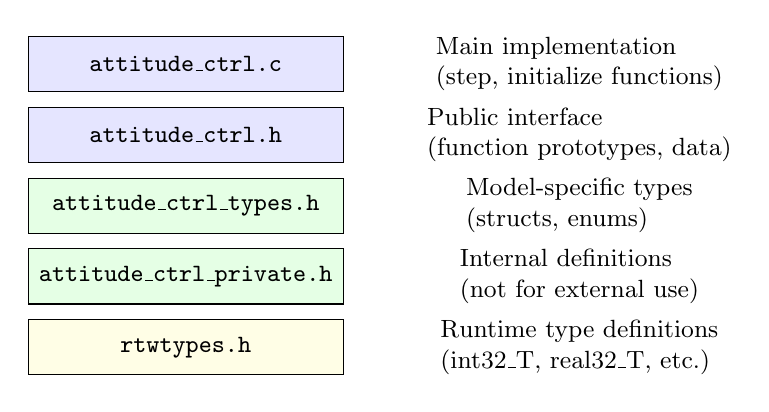
\begin{tikzpicture}[every node/.style={font=\small\ttfamily}]
    \node[draw, rectangle, fill=blue!10, minimum width=4cm, minimum height=0.7cm] (modelc) at (0,0) {attitude\_ctrl.c};
    \node[draw, rectangle, fill=blue!10, minimum width=4cm, minimum height=0.7cm] (modelh) at (0,-0.9) {attitude\_ctrl.h};
    \node[draw, rectangle, fill=green!10, minimum width=4cm, minimum height=0.7cm] (types) at (0,-1.8) {attitude\_ctrl\_types.h};
    \node[draw, rectangle, fill=green!10, minimum width=4cm, minimum height=0.7cm] (private) at (0,-2.7) {attitude\_ctrl\_private.h};
    \node[draw, rectangle, fill=yellow!10, minimum width=4cm, minimum height=0.7cm] (rtw) at (0,-3.6) {rtwtypes.h};

    \node[right of=modelc, xshift=4cm, font=\small\rmfamily, align=left] {Main implementation\\(step, initialize functions)};
    \node[right of=modelh, xshift=4cm, font=\small\rmfamily, align=left] {Public interface\\(function prototypes, data)};
    \node[right of=types, xshift=4cm, font=\small\rmfamily, align=left] {Model-specific types\\(structs, enums)};
    \node[right of=private, xshift=4cm, font=\small\rmfamily, align=left] {Internal definitions\\(not for external use)};
    \node[right of=rtw, xshift=4cm, font=\small\rmfamily, align=left] {Runtime type definitions\\(int32\_T, real32\_T, etc.)};
\end{tikzpicture}
\end{center}

For a model named \texttt{attitude\_ctrl}, you typically get:

\begin{itemize}
    \item \texttt{attitude\_ctrl.c} --- Main source file with algorithm implementation
    \item \texttt{attitude\_ctrl.h} --- Header with public function prototypes and data declarations
    \item \texttt{attitude\_ctrl\_types.h} --- Type definitions used by the model
    \item \texttt{attitude\_ctrl\_private.h} --- Internal macros and definitions
    \item \texttt{rtwtypes.h} --- Portable type definitions (e.g., \texttt{real32\_T} for \texttt{float})
\end{itemize}

\subsection{Entry Point Functions}

Generated code provides three main entry points that your application must call:

\begin{lstlisting}[language=C, caption={The three entry point functions}]
/* Call once at system startup */
void attitude_ctrl_initialize(void);

/* Call once per sample period (e.g., every 2 ms) */
void attitude_ctrl_step(void);

/* Call at shutdown (often empty for embedded systems) */
void attitude_ctrl_terminate(void);
\end{lstlisting}

\paragraph{Initialize Function}
The initialize function sets up initial conditions for all states and parameters:

\begin{lstlisting}[language=C, caption={Typical initialize function structure}]
void attitude_ctrl_initialize(void)
{
    /* Initialize states to their initial values */
    attitude_ctrl_DW.Integrator_DSTATE = 0.0F;
    attitude_ctrl_DW.Filter_DSTATE = 0.0F;

    /* Initialize outputs */
    attitude_ctrl_Y.motor_cmd[0] = 0.0F;
    attitude_ctrl_Y.motor_cmd[1] = 0.0F;
    attitude_ctrl_Y.motor_cmd[2] = 0.0F;
    attitude_ctrl_Y.motor_cmd[3] = 0.0F;
}
\end{lstlisting}

\paragraph{Step Function}
The step function executes one iteration of the control algorithm. This is where the actual computation happens:

\begin{lstlisting}[language=C, caption={Step function structure (simplified)}]
void attitude_ctrl_step(void)
{
    /* Read inputs (populated by calling code) */
    real32_T roll_error = attitude_ctrl_U.roll_setpoint
                        - attitude_ctrl_U.roll_measured;

    /* Compute control law */
    real32_T P_term = attitude_ctrl_P.Kp * roll_error;
    real32_T I_term = attitude_ctrl_DW.Integrator_DSTATE;
    real32_T D_term = attitude_ctrl_P.Kd *
        (roll_error - attitude_ctrl_DW.error_prev);

    /* Update states for next iteration */
    attitude_ctrl_DW.Integrator_DSTATE +=
        attitude_ctrl_P.Ki * roll_error * 0.002F;
    attitude_ctrl_DW.error_prev = roll_error;

    /* Write outputs */
    attitude_ctrl_Y.torque_cmd = P_term + I_term + D_term;
}
\end{lstlisting}

\paragraph{Terminate Function}
For embedded systems running continuously, the terminate function is typically empty or omitted. It exists for completeness and desktop applications that need cleanup.

\subsection{Data Structures}

Generated code organizes data into several global structures. Understanding these structures is key to interfacing with generated code:

\begin{center}
\begin{tikzpicture}[every node/.style={font=\small},
    box/.style={draw, rectangle, minimum width=3.5cm, minimum height=1.2cm, align=center}]

    % External inputs
    \node[box, fill=green!20] (U) at (-4, 2) {\texttt{model\_U}\\External Inputs};

    % Block outputs
    \node[box, fill=blue!20] (B) at (0, 2) {\texttt{model\_B}\\Block Outputs};

    % External outputs
    \node[box, fill=red!20] (Y) at (4, 2) {\texttt{model\_Y}\\External Outputs};

    % States
    \node[box, fill=yellow!20] (DW) at (-2, 0) {\texttt{model\_DW}\\Discrete States};
    \node[box, fill=orange!20] (X) at (2, 0) {\texttt{model\_X}\\Continuous States};

    % Parameters
    \node[box, fill=purple!20] (P) at (0, -2) {\texttt{model\_P}\\Parameters};

    % Arrows showing data flow
    \draw[-{Stealth}, thick] (U) -- (B);
    \draw[-{Stealth}, thick] (B) -- (Y);
    \draw[-{Stealth}, thick] (DW) -- (B);
    \draw[-{Stealth}, thick] (X) -- (B);
    \draw[-{Stealth}, thick] (P) -- (B);
    \draw[-{Stealth}, dashed] (B) to[bend left] (DW);
    \draw[-{Stealth}, dashed] (B) to[bend right] (X);

    \node[below of=P, yshift=0.3cm, font=\footnotesize\itshape] {(Tunable gains, thresholds, etc.)};
\end{tikzpicture}
\end{center}

\paragraph{External Inputs (\texttt{model\_U})}
Structure containing all input signals to the model. Your application populates this before calling the step function:

\begin{lstlisting}[language=C]
typedef struct {
    real32_T roll_setpoint;      /* Desired roll angle [rad] */
    real32_T pitch_setpoint;     /* Desired pitch angle [rad] */
    real32_T yaw_rate_setpoint;  /* Desired yaw rate [rad/s] */
    real32_T roll_measured;      /* Measured roll from estimator */
    real32_T pitch_measured;     /* Measured pitch from estimator */
    real32_T yaw_rate_measured;  /* Measured yaw rate from gyro */
} ExtU_attitude_ctrl_T;

extern ExtU_attitude_ctrl_T attitude_ctrl_U;
\end{lstlisting}

\paragraph{External Outputs (\texttt{model\_Y})}
Structure containing all output signals from the model. Your application reads this after the step function returns:

\begin{lstlisting}[language=C]
typedef struct {
    real32_T motor_cmd[4];  /* Motor commands [0-65535] */
} ExtY_attitude_ctrl_T;

extern ExtY_attitude_ctrl_T attitude_ctrl_Y;
\end{lstlisting}

\paragraph{Discrete Work States (\texttt{model\_DW})}
Structure containing discrete-time states that persist between step function calls:

\begin{lstlisting}[language=C]
typedef struct {
    real32_T Integrator_DSTATE;    /* Integrator state */
    real32_T Filter_DSTATE;        /* Derivative filter state */
    real32_T UnitDelay_DSTATE;     /* Unit delay state */
} DW_attitude_ctrl_T;

extern DW_attitude_ctrl_T attitude_ctrl_DW;
\end{lstlisting}

\paragraph{Continuous States (\texttt{model\_X})}
For models with continuous-time dynamics (using integrators with continuous sample time), states are stored separately:

\begin{lstlisting}[language=C]
typedef struct {
    real32_T Integrator_CSTATE;  /* Continuous integrator state */
} X_attitude_ctrl_T;

extern X_attitude_ctrl_T attitude_ctrl_X;
\end{lstlisting}

\paragraph{Parameters (\texttt{model\_P})}
Structure containing tunable parameters. These can be modified at runtime for calibration:

\begin{lstlisting}[language=C]
typedef struct {
    real32_T Kp_roll;    /* Proportional gain for roll */
    real32_T Ki_roll;    /* Integral gain for roll */
    real32_T Kd_roll;    /* Derivative gain for roll */
    real32_T Kp_pitch;   /* Proportional gain for pitch */
    /* ... more parameters ... */
} P_attitude_ctrl_T;

extern P_attitude_ctrl_T attitude_ctrl_P;
\end{lstlisting}

\begin{notebox}
The parameter structure allows runtime tuning without recompiling. During development, you can adjust gains via a debugger or communication link, then update the model with final values.
\end{notebox}

\section{Block-to-Code Mapping}

Understanding how Simulink blocks translate to C code helps you predict generated code behavior and optimize your models.

\subsection{Gain Block}

A Gain block multiplies its input by a constant:

\begin{minipage}[t]{0.45\textwidth}
\textbf{Simulink Block:}
\begin{center}
\begin{tikzpicture}
    \node[draw, trapezium, trapezium left angle=70, trapezium right angle=110,
          minimum width=1.5cm, minimum height=1cm] (gain) {Kp};
    \draw[-{Stealth}] (-1.5,0) -- (gain.west) node[midway, above] {error};
    \draw[-{Stealth}] (gain.east) -- (2,0) node[midway, above] {P\_term};
\end{tikzpicture}
\end{center}
\end{minipage}
\hfill
\begin{minipage}[t]{0.5\textwidth}
\textbf{Generated Code:}
\begin{lstlisting}[language=C]
/* Gain: '<S1>/Kp' */
rtb_P_term = ctrl_P.Kp * rtb_error;
\end{lstlisting}
\end{minipage}

\subsection{Sum Block}

A Sum block adds or subtracts signals:

\begin{minipage}[t]{0.45\textwidth}
\textbf{Simulink Block:}
\begin{center}
\begin{tikzpicture}
    \node[draw, circle, minimum size=0.8cm] (sum) {};
    \node at (sum.center) {$+$};
    \draw[-{Stealth}] (-1.5,0.3) -- (sum.west) node[midway, above] {setpoint};
    \draw[-{Stealth}] (-1.5,-0.3) -- (sum.west);
    \node at (-1.2,-0.5) {\small $-$};
    \node at (-1.8,-0.3) {measured};
    \draw[-{Stealth}] (sum.east) -- (1.5,0) node[midway, above] {error};
\end{tikzpicture}
\end{center}
\end{minipage}
\hfill
\begin{minipage}[t]{0.5\textwidth}
\textbf{Generated Code:}
\begin{lstlisting}[language=C]
/* Sum: '<S1>/Sum' */
rtb_error = ctrl_U.setpoint
          - ctrl_U.measured;
\end{lstlisting}
\end{minipage}

\subsection{Discrete Integrator}

A discrete integrator accumulates its input over time, implementing $y[k] = y[k-1] + T_s \cdot u[k]$:

\begin{minipage}[t]{0.45\textwidth}
\textbf{Simulink Block:}
\begin{center}
\begin{tikzpicture}
    \node[draw, rectangle, minimum width=2cm, minimum height=1cm] (int) {$\frac{T_s}{z-1}$};
    \draw[-{Stealth}] (-2,0) -- (int.west) node[midway, above] {error};
    \draw[-{Stealth}] (int.east) -- (2,0) node[midway, above] {I\_term};
\end{tikzpicture}
\end{center}
\end{minipage}
\hfill
\begin{minipage}[t]{0.5\textwidth}
\textbf{Generated Code:}
\begin{lstlisting}[language=C]
/* DiscreteIntegrator: '<S1>/I' */
rtb_I_term = ctrl_DW.I_DSTATE;

/* Update for DiscreteIntegrator */
ctrl_DW.I_DSTATE += 0.002F * rtb_error;
\end{lstlisting}
\end{minipage}

\vspace{0.5em}

Note how the output uses the \emph{previous} state value, and the state update happens separately. This ensures correct discrete-time semantics.

\subsection{Discrete Transfer Function}

A discrete transfer function implements a difference equation. For example, a first-order low-pass filter:

$$H(z) = \frac{b_0 + b_1 z^{-1}}{1 + a_1 z^{-1}}$$

\begin{lstlisting}[language=C, caption={Generated code for discrete transfer function}]
/* DiscreteTransferFcn: '<S1>/LowPass' */
{
    real32_T denAccum;
    real32_T numAccum;

    /* Denominator: 1 + a1*z^(-1) */
    denAccum = ctrl_U.input - ctrl_P.LowPass_DenCoef[1]
             * ctrl_DW.LowPass_states;

    /* Numerator: b0 + b1*z^(-1) */
    numAccum = ctrl_P.LowPass_NumCoef[0] * denAccum
             + ctrl_P.LowPass_NumCoef[1] * ctrl_DW.LowPass_states;

    /* Update state */
    ctrl_DW.LowPass_states = denAccum;

    rtb_filtered = numAccum;
}
\end{lstlisting}

\subsection{Saturation Block}

A Saturation block limits its input to a specified range:

\begin{minipage}[t]{0.45\textwidth}
\textbf{Simulink Block:}
\begin{center}
\begin{tikzpicture}
    \node[draw, rectangle, minimum width=1.8cm, minimum height=1cm] (sat) {};
    \draw[thick] (-0.5,-0.3) -- (-0.2,-0.3) -- (0.2,0.3) -- (0.5,0.3);
    \draw[-{Stealth}] (-2,0) -- (sat.west) node[midway, above] {cmd};
    \draw[-{Stealth}] (sat.east) -- (2,0) node[midway, above] {cmd\_sat};
\end{tikzpicture}
\end{center}
\end{minipage}
\hfill
\begin{minipage}[t]{0.5\textwidth}
\textbf{Generated Code:}
\begin{lstlisting}[language=C]
/* Saturation: '<S1>/Sat' */
if (rtb_cmd > ctrl_P.Sat_UpperLimit) {
    rtb_cmd_sat = ctrl_P.Sat_UpperLimit;
} else if (rtb_cmd < ctrl_P.Sat_LowerLimit) {
    rtb_cmd_sat = ctrl_P.Sat_LowerLimit;
} else {
    rtb_cmd_sat = rtb_cmd;
}
\end{lstlisting}
\end{minipage}

\subsection{Stateflow Chart}

Stateflow charts generate state machine code using switch-case structures:

\begin{lstlisting}[language=C, caption={Generated code for a flight mode state machine}]
void FlightMode_step(void)
{
    /* Chart: '<Root>/FlightMode' */
    switch (FlightMode_DW.is_c1_FlightMode) {
      case IN_Idle:
        if (FlightMode_U.arm_cmd) {
            FlightMode_DW.is_c1_FlightMode = IN_Armed;
            FlightMode_Y.motors_enabled = false;
        }
        break;

      case IN_Armed:
        if (FlightMode_U.takeoff_cmd) {
            FlightMode_DW.is_c1_FlightMode = IN_Flying;
            FlightMode_Y.motors_enabled = true;
        } else if (!FlightMode_U.arm_cmd) {
            FlightMode_DW.is_c1_FlightMode = IN_Idle;
        }
        break;

      case IN_Flying:
        if (FlightMode_U.land_cmd) {
            FlightMode_DW.is_c1_FlightMode = IN_Landing;
        }
        break;

      case IN_Landing:
        if (FlightMode_U.landed) {
            FlightMode_DW.is_c1_FlightMode = IN_Armed;
            FlightMode_Y.motors_enabled = false;
        }
        break;
    }
}
\end{lstlisting}

\begin{keyidea}
Stateflow generates deterministic, efficient state machine code using enumerated states and switch-case logic. This is more maintainable than hand-coding complex state transitions.
\end{keyidea}

\section{Model Configuration for Embedded Systems}

Proper configuration is essential for generating efficient, correct embedded code.

\subsection{Hardware Implementation Settings}

The Hardware Implementation pane specifies target processor characteristics:

\begin{center}
\begin{tabular}{ll}
\toprule
\textbf{Setting} & \textbf{Value for STM32F4} \\
\midrule
Device vendor & ARM Compatible \\
Device type & ARM Cortex-M \\
Byte ordering & Little Endian \\
Signed integer division rounds to & Zero \\
Native word size & 32 bits \\
\texttt{char} size & 8 bits \\
\texttt{short} size & 16 bits \\
\texttt{int} size & 32 bits \\
\texttt{long} size & 32 bits \\
\texttt{float} size & 32 bits \\
\texttt{double} size & 64 bits \\
\bottomrule
\end{tabular}
\end{center}

These settings affect code generation choices like data type selection and arithmetic operations.

\subsection{Code Generation Options}

Key options in the Code Generation pane:

\paragraph{System Target File}
Specifies the target configuration. For Embedded Coder:
\begin{itemize}
    \item \texttt{ert.tlc} --- Generic Embedded Real-Time target
    \item Custom targets for specific hardware (e.g., STM32)
\end{itemize}

\paragraph{Code Interface}
\begin{itemize}
    \item \textbf{Nonreusable function} --- Single instance, global data (simpler)
    \item \textbf{Reusable function} --- Multiple instances, passed data (more flexible)
\end{itemize}

For a single quadrotor, nonreusable functions are simpler. Reusable functions are useful when you need multiple instances of the same controller.

\paragraph{Optimization Level}
\begin{itemize}
    \item \textbf{Minimum} --- Most readable code, useful for debugging
    \item \textbf{Maximum} --- Most efficient code, aggressive inlining
\end{itemize}

\paragraph{Comments}
Enable \textbf{Include comments} and \textbf{Simulink block comments} for traceability. Each line of generated code includes a comment identifying the source block:

\begin{lstlisting}[language=C]
/* Gain: '<S1>/Kp' incorporates:
 *  Sum: '<S1>/Sum' */
rtb_P_term = ctrl_P.Kp * (ctrl_U.setpoint - ctrl_U.measured);
\end{lstlisting}

\subsection{Fixed-Point vs Floating-Point}

The STM32F405 has a hardware floating-point unit (FPU), so single-precision floating-point is efficient. However, some applications benefit from fixed-point:

\begin{center}
\begin{tabular}{lll}
\toprule
\textbf{Aspect} & \textbf{Floating-Point} & \textbf{Fixed-Point} \\
\midrule
Dynamic range & Very large & Limited by word size \\
Precision & Relative (6-7 digits) & Absolute (fixed) \\
Hardware support & FPU required & Integer ALU \\
Code portability & Universal & May need tuning \\
Development effort & Lower & Higher \\
\bottomrule
\end{tabular}
\end{center}

For the Crazyflie, single-precision floating-point (\texttt{float}, \texttt{real32\_T}) is recommended because:
\begin{itemize}
    \item The Cortex-M4F has hardware single-precision FPU
    \item Control calculations fit comfortably in 32-bit float range
    \item Development time is significantly reduced
\end{itemize}

\begin{warningbox}
Avoid double-precision (\texttt{double}) on the STM32F4. The FPU only supports single-precision, so double operations fall back to slow software emulation.
\end{warningbox}

\subsection{Memory Allocation}

For safety-critical embedded systems, static memory allocation is preferred:

\begin{itemize}
    \item \textbf{Static allocation}: All memory allocated at compile time
    \begin{itemize}
        \item Predictable memory footprint
        \item No fragmentation
        \item No runtime allocation failures
    \end{itemize}

    \item \textbf{Dynamic allocation}: Memory allocated via \texttt{malloc()}
    \begin{itemize}
        \item Flexible but unpredictable
        \item Risk of fragmentation
        \item Risk of allocation failure
    \end{itemize}
\end{itemize}

Configure Embedded Coder to use static allocation by enabling \textbf{Static code} in the Code Generation $\rightarrow$ Interface settings.

\section{Integration with Hand-Written Code}

Generated code must integrate with your existing firmware---sensor drivers, communication stacks, and RTOS infrastructure.

\subsection{Calling Generated Code from Main}

The basic integration pattern places generated code in your main control loop:

\begin{lstlisting}[language=C, caption={Integrating generated code with FreeRTOS}]
#include "attitude_ctrl.h"
#include "sensors.h"
#include "motors.h"

void attitudeControlTask(void *pvParameters)
{
    TickType_t xLastWakeTime = xTaskGetTickCount();
    const TickType_t xPeriod = pdMS_TO_TICKS(2);  /* 500 Hz */

    /* Initialize the generated code */
    attitude_ctrl_initialize();

    for (;;) {
        /* Wait for next period */
        vTaskDelayUntil(&xLastWakeTime, xPeriod);

        /* Read sensors and populate inputs */
        SensorData_t sensors = readIMU();
        attitude_ctrl_U.roll_measured = sensors.roll;
        attitude_ctrl_U.pitch_measured = sensors.pitch;
        attitude_ctrl_U.yaw_rate_measured = sensors.gyro_z;

        /* Get setpoints from commander */
        attitude_ctrl_U.roll_setpoint = getSetpoint(ROLL);
        attitude_ctrl_U.pitch_setpoint = getSetpoint(PITCH);
        attitude_ctrl_U.yaw_rate_setpoint = getSetpoint(YAW_RATE);

        /* Execute one step of the controller */
        attitude_ctrl_step();

        /* Apply outputs to motors */
        setMotorCommands(attitude_ctrl_Y.motor_cmd);
    }
}
\end{lstlisting}

\subsection{S-Functions for Custom Blocks}

When you need functionality not available in standard Simulink blocks, S-functions let you write custom blocks in C:

\begin{lstlisting}[language=C, caption={S-function wrapper for custom sensor driver}]
/* S-function: ReadIMU */
static void mdlOutputs(SimStruct *S, int_T tid)
{
    real32_T *roll  = (real32_T *)ssGetOutputPortSignal(S, 0);
    real32_T *pitch = (real32_T *)ssGetOutputPortSignal(S, 1);
    real32_T *yaw   = (real32_T *)ssGetOutputPortSignal(S, 2);

    /* Call the actual sensor driver */
    SensorData_t data = readIMU();

    *roll  = data.roll;
    *pitch = data.pitch;
    *yaw   = data.yaw;
}
\end{lstlisting}

During simulation, the S-function can provide simulated sensor data. For code generation, it produces calls to your actual driver functions.

\subsection{Legacy Code Tool}

The Legacy Code Tool automates wrapping existing C code as Simulink blocks:

\begin{lstlisting}[language=matlab, caption={Using Legacy Code Tool in MATLAB}]
% Define the legacy function interface
def = legacy_code('initialize');
def.SFunctionName = 'sfun_motor_mixer';
def.HeaderFiles = {'motor_mixer.h'};
def.SourceFiles = {'motor_mixer.c'};
def.OutputFcnSpec = ...
    'void motor_mix(single u1[4], single y1[4])';

% Generate the S-function
legacy_code('sfcn_cmex_generate', def);
legacy_code('compile', def);
legacy_code('slblock_generate', def);
\end{lstlisting}

This creates a Simulink block that calls your existing \texttt{motor\_mix()} function, both in simulation and in generated code.

\subsection{External Mode for Parameter Tuning}

External mode enables live parameter tuning while the generated code runs on target:

\begin{center}
\begin{tikzpicture}[every node/.style={font=\small}]
    \node[draw, rectangle, rounded corners, fill=blue!10, minimum width=3cm, minimum height=1.5cm, align=center] (sim) at (0,0) {Simulink\\(Host PC)};
    \node[draw, rectangle, rounded corners, fill=green!10, minimum width=3cm, minimum height=1.5cm, align=center] (target) at (6,0) {Generated Code\\(STM32)};

    \draw[{Stealth}-{Stealth}, thick] (sim) -- (target)
        node[midway, above] {Serial/USB}
        node[midway, below] {Parameter changes};
\end{tikzpicture}
\end{center}

In External mode:
\begin{enumerate}
    \item Simulink connects to the running target via serial or USB
    \item Changing a parameter in Simulink updates the target's \texttt{model\_P} structure
    \item Signal values can be monitored and logged from the target
\end{enumerate}

This is invaluable for tuning control gains on the actual hardware.

\section{Real-Time Execution Considerations}

Generated code must execute within strict timing constraints. This section connects code generation to the real-time concepts from Module~3.

\subsection{Single-Rate vs Multi-Rate Models}

\paragraph{Single-Rate Models}
All blocks execute at the same rate. Generated code has a single \texttt{model\_step()} function:

\begin{lstlisting}[language=C]
/* Single-rate: everything at 500 Hz */
void control_step(void)
{
    /* All computations here */
}
\end{lstlisting}

\paragraph{Multi-Rate Models}
Blocks execute at different rates. Generated code has rate-specific step functions:

\begin{lstlisting}[language=C]
/* Multi-rate: 500 Hz and 100 Hz */
void control_step0(void)  /* Fast rate: 500 Hz */
{
    /* Attitude control */
}

void control_step1(void)  /* Slow rate: 100 Hz */
{
    /* Position control */
}
\end{lstlisting}

The calling code must invoke each step function at the correct rate:

\begin{lstlisting}[language=C, caption={Scheduling multi-rate generated code}]
static uint32_t tick_count = 0;

void timerISR(void)
{
    tick_count++;

    /* Fast rate: every tick (2 ms = 500 Hz) */
    control_step0();

    /* Slow rate: every 5 ticks (10 ms = 100 Hz) */
    if ((tick_count % 5) == 0) {
        control_step1();
    }
}
\end{lstlisting}

\subsection{Overrun Detection}

If the step function takes longer than the sample period, you have a timing overrun:

\begin{lstlisting}[language=C, caption={Detecting timing overruns}]
volatile uint32_t overrun_count = 0;
volatile bool step_in_progress = false;

void timerISR(void)
{
    if (step_in_progress) {
        /* Previous step didn't complete in time! */
        overrun_count++;
        return;  /* Skip this step or handle error */
    }

    step_in_progress = true;
    control_step();
    step_in_progress = false;
}
\end{lstlisting}

\begin{warningbox}
Timing overruns can cause instability in your control system. Always verify that worst-case execution time is less than the sample period. Use the profiling techniques from Chapter~\ref{ch:rtos} to measure actual execution times.
\end{warningbox}

\subsection{Execution Time Profiling}

Measure generated code execution time to verify timing constraints:

\begin{lstlisting}[language=C, caption={Profiling step function execution time}]
#include "stm32f4xx.h"  /* For DWT cycle counter */

void profile_step(void)
{
    /* Enable cycle counter */
    CoreDebug->DEMCR |= CoreDebug_DEMCR_TRCENA_Msk;
    DWT->CYCCNT = 0;
    DWT->CTRL |= DWT_CTRL_CYCCNTENA_Msk;

    uint32_t start = DWT->CYCCNT;
    control_step();
    uint32_t end = DWT->CYCCNT;

    uint32_t cycles = end - start;
    float microseconds = cycles / 168.0f;  /* 168 MHz clock */

    /* Log or transmit timing data */
    printf("Step time: %.1f us\n", microseconds);
}
\end{lstlisting}

For a 500\,Hz controller, the step function must complete in under 2000\,$\mu$s. In practice, aim for much less (e.g., 500\,$\mu$s) to leave margin for interrupt handling and other tasks.

\section{Verification and Traceability}

Code generation enables systematic verification through the development process.

\subsection{Code-to-Model Traceability}

With comments enabled, every line of generated code traces back to its source block:

\begin{lstlisting}[language=C]
/* Gain: '<S2>/Kp_roll' incorporates:
 *  Inport: '<Root>/roll_error'
 */
ctrl_B.P_term_roll = ctrl_P.Kp_roll * ctrl_U.roll_error;
\end{lstlisting}

The comment \texttt{'<S2>/Kp\_roll'} identifies:
\begin{itemize}
    \item \texttt{S2} --- Subsystem 2 in the model hierarchy
    \item \texttt{Kp\_roll} --- The block name
\end{itemize}

In Simulink, you can navigate from code to model (and vice versa) using the code traceability report.

\subsection{Testing Levels with Generated Code}

Generated code supports multiple testing levels as discussed in Module~4:

\begin{center}
\begin{tabular}{lll}
\toprule
\textbf{Level} & \textbf{Code} & \textbf{Plant} \\
\midrule
MIL & Simulink model & Simulink model \\
SIL & Generated C (on host) & Simulink model \\
PIL & Generated C (on target) & Simulink model \\
HIL & Generated C (on target) & Hardware simulator \\
\bottomrule
\end{tabular}
\end{center}

\paragraph{Software-in-the-Loop (SIL)}
The generated code compiles and runs on the host PC, connected to the Simulink plant model. This verifies the generated code matches the model behavior:

\begin{lstlisting}[language=matlab, caption={Running SIL simulation in MATLAB}]
% Configure for SIL
set_param('attitude_ctrl', 'SimulationMode', 'software-in-the-loop');

% Run simulation
sim('attitude_ctrl');

% Compare outputs
max_error = max(abs(yout_model - yout_sil));
assert(max_error < 1e-6, 'SIL mismatch detected');
\end{lstlisting}

\paragraph{Processor-in-the-Loop (PIL)}
The generated code runs on the actual target processor (STM32), communicating with the Simulink plant model via serial link. This catches issues related to:
\begin{itemize}
    \item Target-specific numerical behavior
    \item Compiler optimizations
    \item Fixed-point overflow (if using fixed-point)
\end{itemize}

\subsection{Code Coverage}

Embedded Coder can generate instrumented code that tracks coverage:

\begin{itemize}
    \item \textbf{Statement coverage}: Which lines executed
    \item \textbf{Decision coverage}: Which branches taken
    \item \textbf{Condition coverage}: Which Boolean sub-expressions evaluated
    \item \textbf{MC/DC}: Modified Condition/Decision Coverage for safety-critical systems
\end{itemize}

Coverage data from PIL tests can satisfy DO-178C or ISO~26262 requirements for safety-critical software.

\section{Practical Example: Attitude Controller}

Let's walk through a complete example of generating code for a PD attitude controller.

\subsection{The Simulink Model}

Consider a simple PD roll controller:

\begin{center}
\begin{tikzpicture}[every node/.style={font=\small}, scale=0.9]
    % Input ports
    \node[draw, rectangle, minimum height=0.6cm] (sp) at (-5, 0.5) {setpoint};
    \node[draw, rectangle, minimum height=0.6cm] (meas) at (-5, -0.5) {measured};

    % Sum
    \node[draw, circle, minimum size=0.6cm] (sum) at (-3, 0) {};
    \node at (-3, 0) {$\Sigma$};

    % Gains
    \node[draw, trapezium, trapezium left angle=70, trapezium right angle=110,
          minimum width=1cm] (kp) at (-0.5, 0.5) {Kp};
    \node[draw, trapezium, trapezium left angle=70, trapezium right angle=110,
          minimum width=1cm] (kd) at (-0.5, -0.5) {Kd};

    % Derivative
    \node[draw, rectangle, minimum width=1.2cm] (deriv) at (-0.5, -1.5) {$\frac{N}{1+N/s}$};

    % Output sum
    \node[draw, circle, minimum size=0.6cm] (outsum) at (2, 0) {};
    \node at (2, 0) {$\Sigma$};

    % Output
    \node[draw, rectangle, minimum height=0.6cm] (out) at (4, 0) {torque};

    % Connections
    \draw[-{Stealth}] (sp) -| (-3.3, 0.3);
    \draw[-{Stealth}] (meas) -| (-3.3, -0.3);
    \draw[-{Stealth}] (sum) -- (-1.5, 0) node[midway, above] {error};
    \draw[-{Stealth}] (-1.5, 0) |- (kp);
    \draw[-{Stealth}] (-1.5, 0) |- (deriv);
    \draw[-{Stealth}] (deriv) -- (kd);
    \draw[-{Stealth}] (kp) -| (1.7, 0.3);
    \draw[-{Stealth}] (kd) -| (1.7, -0.3);
    \draw[-{Stealth}] (outsum) -- (out);

    \node at (-3, -0.5) {\tiny $-$};
\end{tikzpicture}
\end{center}

The model uses a filtered derivative (transfer function $\frac{Ns}{s+N}$) to avoid amplifying noise.

\subsection{Generated File Structure}

After code generation, you get:

\begin{verbatim}
roll_ctrl/
  roll_ctrl.c           # Main implementation
  roll_ctrl.h           # Public interface
  roll_ctrl_types.h     # Data types
  roll_ctrl_private.h   # Internal definitions
  rtwtypes.h            # Runtime types
  roll_ctrl_data.c      # Parameter initialization
\end{verbatim}

\subsection{Key Generated Code}

\paragraph{Data Structures}

\begin{lstlisting}[language=C, caption={Generated data structures}]
/* External inputs */
typedef struct {
    real32_T setpoint;   /* '<Root>/setpoint' */
    real32_T measured;   /* '<Root>/measured' */
} ExtU_roll_ctrl_T;

/* External outputs */
typedef struct {
    real32_T torque;     /* '<Root>/torque' */
} ExtY_roll_ctrl_T;

/* Block states (discrete work) */
typedef struct {
    real32_T Filter_DSTATE;  /* '<S1>/Filter' (derivative filter) */
} DW_roll_ctrl_T;

/* Parameters */
typedef struct {
    real32_T Kp;         /* Variable: Kp */
    real32_T Kd;         /* Variable: Kd */
    real32_T N;          /* Variable: N (filter coefficient) */
} P_roll_ctrl_T;

/* Global instances */
extern ExtU_roll_ctrl_T roll_ctrl_U;
extern ExtY_roll_ctrl_T roll_ctrl_Y;
extern DW_roll_ctrl_T roll_ctrl_DW;
extern P_roll_ctrl_T roll_ctrl_P;
\end{lstlisting}

\paragraph{Initialize Function}

\begin{lstlisting}[language=C, caption={Generated initialize function}]
void roll_ctrl_initialize(void)
{
    /* Initialize states */
    roll_ctrl_DW.Filter_DSTATE = 0.0F;

    /* Initialize outputs */
    roll_ctrl_Y.torque = 0.0F;
}
\end{lstlisting}

\paragraph{Step Function}

\begin{lstlisting}[language=C, caption={Generated step function}]
void roll_ctrl_step(void)
{
    real32_T rtb_error;
    real32_T rtb_FilteredDerivative;

    /* Sum: '<S1>/Sum' */
    rtb_error = roll_ctrl_U.setpoint - roll_ctrl_U.measured;

    /* DiscreteTransferFcn: '<S1>/Filter'
     * Implements filtered derivative: N*s/(s+N) discretized */
    rtb_FilteredDerivative = roll_ctrl_P.N * rtb_error
                           - roll_ctrl_P.N * roll_ctrl_DW.Filter_DSTATE;

    /* Update for DiscreteTransferFcn: '<S1>/Filter' */
    roll_ctrl_DW.Filter_DSTATE = (2.0F - roll_ctrl_P.N * 0.002F)
        / (2.0F + roll_ctrl_P.N * 0.002F) * roll_ctrl_DW.Filter_DSTATE
        + 0.002F / (2.0F + roll_ctrl_P.N * 0.002F)
        * (rtb_error + roll_ctrl_DW.Filter_prev);
    roll_ctrl_DW.Filter_prev = rtb_error;

    /* Sum: '<S1>/Sum1' incorporates:
     *  Gain: '<S1>/Kp'
     *  Gain: '<S1>/Kd' */
    roll_ctrl_Y.torque = roll_ctrl_P.Kp * rtb_error
                       + roll_ctrl_P.Kd * rtb_FilteredDerivative;
}
\end{lstlisting}

\subsection{Integration into Crazyflie Firmware}

\begin{lstlisting}[language=C, caption={Integrating generated controller into Crazyflie}]
/* In stabilizer.c or equivalent */
#include "roll_ctrl.h"

void stabilizerInit(void)
{
    /* Initialize generated controller */
    roll_ctrl_initialize();

    /* Set initial parameters (can be tuned later) */
    roll_ctrl_P.Kp = 3.5f;
    roll_ctrl_P.Kd = 0.1f;
    roll_ctrl_P.N = 100.0f;
}

void stabilizerTask(void *param)
{
    /* ... task setup ... */

    while (1) {
        vTaskDelayUntil(&lastWakeTime, M2T(2));  /* 500 Hz */

        /* Get sensor data */
        sensorsAcquire(&sensorData);
        stateEstimator(&state, &sensorData);

        /* Populate generated code inputs */
        roll_ctrl_U.setpoint = commanderGetRoll();
        roll_ctrl_U.measured = state.attitude.roll;

        /* Execute generated controller */
        roll_ctrl_step();

        /* Use output */
        controlOutput.roll_torque = roll_ctrl_Y.torque;

        /* ... similar for pitch and yaw ... */

        /* Apply to motors via mixer */
        powerDistribution(&controlOutput, motorCommands);
    }
}
\end{lstlisting}

\begin{keyidea}
The generated code becomes a modular component in your firmware. The interface is well-defined (inputs, outputs, parameters), making it easy to swap different controller designs or update the model.
\end{keyidea}

\section{Summary}

This appendix covered the essentials of Simulink code generation:

\begin{itemize}
    \item \textbf{Workflow}: Model $\rightarrow$ TLC $\rightarrow$ C code $\rightarrow$ Cross-compile $\rightarrow$ Binary
    \item \textbf{Configuration}: Fixed-step solver, hardware settings, optimization options
    \item \textbf{Code structure}: Initialize/step/terminate functions, data structures (U, Y, DW, P)
    \item \textbf{Block mapping}: How Simulink blocks become C operations
    \item \textbf{Integration}: Calling generated code from your main loop or RTOS tasks
    \item \textbf{Real-time}: Managing multi-rate execution and detecting overruns
    \item \textbf{Verification}: Traceability, SIL/PIL testing, coverage analysis
\end{itemize}

Code generation bridges the gap between model-based design and embedded implementation. By understanding the generated code structure, you can effectively integrate auto-generated controllers with hand-written firmware, verify correct operation across testing levels, and deploy verified software to your quadrotor.

\begin{notebox}
The examples in this appendix use simplified code for clarity. Actual generated code includes additional features like overflow protection, rate transition blocks for multi-rate systems, and extensive comments for traceability.
\end{notebox}
\index{Simulink!code generation|)}
\index{code generation!Simulink|)}
